\documentclass[12pt,twoside,openright]{report}

% Hyperlink references
\usepackage[pdfborder={0 0 0}]{hyperref}
% PGF diagrams
\usepackage{pgf}
\usepackage[utf8]{inputenc}\DeclareUnicodeCharacter{2212}{-}
% Page margins
\usepackage[margin=25mm]{geometry}
% Subfigures
\usepackage{caption}
\usepackage{subcaption}
% Bibliography
\usepackage[style=numeric-comp,sorting=none]{biblatex}
% Images
\usepackage{graphicx}
% Directory tree diagram
\usepackage{dirtree}
% Simple tree diagrams
\usepackage[linguistics]{forest}
\usepackage{adjustbox}
% Algorithms
\usepackage[ruled]{algorithm2e}
% Verbatim++
\usepackage{alltt}
% Text colour
\usepackage{xcolor}
% Better verbatim
\usepackage{fancyvrb}
% TikZ diagrams
\usepackage{tikz}
% UK date
\usepackage[UKenglish]{babel}
\usepackage{csquotes}
% Paragraph spacing
\usepackage{parskip}
% Verbatim in caption
\usepackage{cprotect}

\addbibresource{bibliography.bib}

%\renewcommand{\baselinestretch}{1.1}
\raggedbottom

\DeclareRobustCommand{\setmetre}[2]{\ensuremath{
  \vcenter{\offinterlineskip
    \halign{\hfil##\hfil\cr
            $\scriptstyle#1$\cr
            \noalign{\vskip1pt}
            $\scriptstyle#2$\cr}
  }}
}

\definecolor{SPpink}{RGB}{255,20,147}
\definecolor{SPblue}{RGB}{30,144,255}
\definecolor{SPorange}{RGB}{255,140,0}
\definecolor{SPgreen}{RGB}{97,206,60}

\begin{document}

%%%%%%%%%%%%%%%%%%%%%%%%%%%%%%%%%%%%%%%%%%%%%%%%%%%%%%%%%%%%%%%%%%%%%%%%
% Title

\begin{titlepage}
    \pagestyle{empty}

    \rightline{\LARGE \textbf{Max Johnson}}

    \vspace*{60mm}
    \begin{center}
    \Huge
    \textbf{Musical micro-timing for live coding} \\[5mm]
    Computer Science Tripos -- Part II \\[5mm]
    Clare College \\[5mm]
    \today
    \end{center}
\end{titlepage}

%%%%%%%%%%%%%%%%%%%%%%%%%%%%%%%%%%%%%%%%%%%%%%%%%%%%%%%%%%%%%%%%%%%%%%%%
% Proforma, table of contents and list of figures

\pagestyle{plain}

\section*{Declaration}

I, [Name] of [College], being a candidate for Part II of the Computer Science Tripos, hereby declare that this dissertation and the work described in it are my own work, unaided except as may be specified below, and that the dissertation does not contain material that has already been used to any substantial extent for a comparable purpose. I am content for my dissertation to be made available to the students and staff of the University.

\bigskip
\leftline{Signed [signature]}

\medskip
\leftline{Date [date]}


\newpage
\chapter*{Proforma}

{\large
\begin{tabular}{ll}
Name:               & \bf Max Johnson                       \\
College:            & \bf Clare College                     \\
Project Title:      & \bf Musical micro-timing for live coding \\
Examination:        & \bf Computer Science Tripos -- Part II, July 2022  \\
Word Count:         & \bf N/A \\
Project Originator: & Mark Gotham                    \\
Supervisor:         & Mark Gotham                    \\ 
\end{tabular}
}


\section*{Original aims of the project}

TBC


\section*{Work completed}

TBC

\section*{Special difficulties}

TBC
 
\newpage
\tableofcontents

%%%%%%%%%%%%%%%%%%%%%%%%%%%%%%%%%%%%%%%%%%%%%%%%%%%%%%%%%%%%%%%%%%%%%%%

\pagestyle{headings}

\chapter{Introduction}

Text.



\chapter{Preparation}

This chapter will introduce the core theories and background material necessary
to understand the project. I will explain some key concepts in music theory and
live coding and give an overview of the case study musical styles. Next, I will
describe the starting point of this project, expand upon the requirements from
the project proposal, and conclude with an outline of the software engineering
techniques used throughout.



\section{Background} \label{background}


\subsection{Musical metre} \label{metre_background}

A beat is a regularly occurring pulse in music. This is usually the pulse you
might tap your foot along to when listening to a piece of music. Musical metre
describes the ways in which beats are grouped and divided within recurring
cycles. This forms different metrical levels within a hierarchy. Division levels
are ones where the beat has been divided into more, shorter durations. Multiple
levels are ones where the beats are grouped into fewer, longer durations. Figure~\ref{fig:metre_hierarchy_example} 
shows the beat level, and some of the division and multiple levels for a simple \ \setmetre{4}{4} time signature, as well as a tree representation of the metrical hierarchy.
A metre is `simple' if its first division level splits the beat into two, and
`compound' if it splits into three \cite{omt2021}.

\begin{figure}
    \centering
    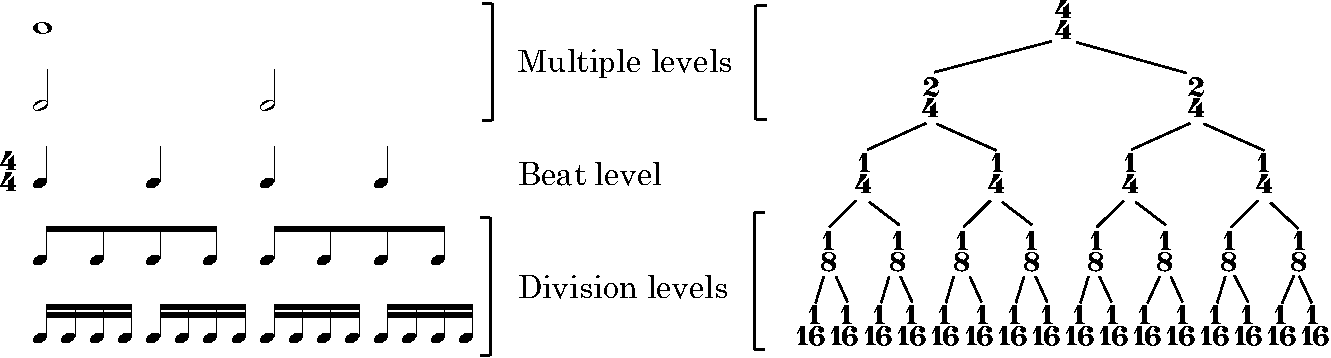
\includegraphics[width=\linewidth]{figures/metre_example.pdf}
    \caption{Example metrical hierarchy for the \setmetre{4}{4} time signature. Left: The hierarchy as notes in traditional Western music notation. Right: The hierarchy as a tree of durations.}
    \label{fig:metre_hierarchy_example}
\end{figure}

Every note in a piece of music occurs at a particular metrical position, but
music performed by humans often deviates from these mechanically even timings
\cite{london2012}. The ways in which these deviations occur contribute significantly
to what we call musical style by producing micro-timing effects. Different
musical styles have different micro-timing strategies. A common example is the
long-short pattern in swing rhythms, where every other eighth note (the first
division level) is slightly delayed. This timing information is typically lost
in music notation \textcolor{red}{(see FIGURE for an example of this)}, so musicians have to use
their knowledge and experience of the style to inform their performance of the
micro-timing. This is formalised in Justin London's Many Meters Hypothesis
\cite{london2012}. A metre without any micro-timing is said to be `isochronous',
which means the metric events at each level are equally spaced in time.


\subsection{Live coding} \label{live_coding_background}

Music live coding is a way of creating and performing music by writing and
modifying code in real time. The performer typically projects their code onto a
screen for an audience to follow along with \cite{magnusson2011}. The liveness of the
performance is important -- it is argued that the musician must directly
interact with the running algorithms for it to be truly considered live coding
\cite{collins2011}. Otherwise, there is little difference between this and playing a
recording of synthesised music.

Sonic Pi is a popular live coding language and IDE created by Sam Aaron, which
was designed as an educational tool for teaching programming in schools. It
implements its own domain-specific language written in Ruby, using the
SuperCollider sound synthesis server to produce sounds \cite{aaron2013}. A simple
Sonic Pi program might look like the following:

\begin{BVerbatim}[commandchars=\\\{\}]
play \textcolor{SPpink}{:C4}
sleep(\textcolor{SPblue}{1})
play \textcolor{SPpink}{:C5}
sleep(\textcolor{SPblue}{0.5})
play \textcolor{SPpink}{:C4}
\end{BVerbatim}

This plays the note C4 on the current synthesiser, sleeps for one beat, plays C5,
sleeps for half a beat, then plays C4 again.

A key component of the Sonic Pi language is the \verb'live_loop', which executes a
block of code in a loop in a new thread. This multi-threading allows multiple
musical parts/instruments to be played together. To maintain correct timing in the presence
of multiple threads and long execution time, Sonic Pi uses sophisticated
``virtual time'' functionality behind-the-scenes \cite{aaron2014}.

One drawback of Sonic Pi is that it currently doesn't have a built-in notion of
metre or style-specific micro-timing, which is what this project addresses.


\subsection{Case studies} \label{case_studies}

This project uses two different styles of music as case studies for evaluation,
both of which have well-known micro-timing characteristics. The first is jembe
drum music from Mali, which has highly regular micro-timing, and the second is
Viennese waltz music, which offers a Western comparison.

Jembe ensemble music is a style of music involving a small group of drummers
which originated in West Africa. The primary drum is the eponymous jembe, which
is a goblet-shaped drum played with the bare hands. This is usually accompanied
by the dundun, which is a cylindrical drum played with a stick \cite{polak2010}. In a
traditional jembe trio, there are two jembe players and one dundun player, with
Jembe 1 having a lead role, Jembe 2 playing a simple accompaniment, and Dundun
playing a varying pattern that is characteristic of each piece of music
\cite{jacoby2021}. Different playing techniques produce various kinds of sound
(timbre) on each drum, which gives rise to the melodic qualities of the music
\cite{polak2010}.

Jembe music is an ideal case study for this project because it has a highly
consistent micro-timing strategy \cite{polak2010}, and Malian drummers have been shown to
have one of the lowest levels of timing variability between performers in the
world \cite{clayton2020}. Compared with other styles of music, jembe music is
relatively constrained in terms of its pitch, timbre, and number of instruments,
which allows for a clear focus on timing.

The Viennese waltz is a style of music intended for ballroom dancing. It is a
fast waltz in \setmetre{3}{4} at around 180 beats per minute (bpm) and is performed by a
classical Western orchestra. It has a characteristic short-long-long
micro-timing pattern for the length of its beats \cite{bengtsson1974,bengtsson1977}.



\section{Starting point} \label{starting_point}

The main implementation of this project is built on top of Sonic Pi, which
handles audio synthesis, sample playback, timekeeping, basic multi-threading,
and all lower-level software components. It includes a simple representation of
beats (although this acts more as a virtual clock than beats in a metrical sense)
and tempo but has no support for metre.

Otherwise:
\begin{itemize}
	\item No work towards this project had been started in advance
	\item Data analysis of recordings of jembe music used existing datasets
	\item I had previous experience of using the Python programming language
	\item Common software libraries such as pandas and Matplotlib were used
	\item I had previous knowledge of basic music theory concepts
\end{itemize}



\section{Requirements analysis} \label{requirements_analysis}

The project proposal (SECTION) features a list of success criteria outlining the
key milestones that needed to be achieved for the project to succeed. It also
has a description of possible extensions. During the research and investigation
stage of the project, I refined these into the list of requirements shown in
Table~\ref{table:requirements}.

\begin{table}
\centering
\begin{tabular}{|l|c|}
    \hline
    \textbf{Requirement}                                      & \textbf{Priority} \\
    \hline
    Research and implement representation of musical metre              & High \\
    Implement commands to play music in a given metre                   & High \\
    Implement representation of probability distributions for a style   & High \\
    Use distributions to implement probabilistic micro-timing           & High \\
    Perform data analysis on jembe recording dataset                    & High \\
    Perform data analysis on Viennese waltz recordings                  & Medium \\
    Generate synthetic music for the jembe case study                   & High \\
    Conduct user study to evaluate realism of generated music           & High \\
    Implement converter to and from MusicXML                            & Low \\
    \hline
\end{tabular}
\caption{Refined list of requirements (and their priorities) that should be achieved for the project to succeed as planned}
\label{table:requirements}
\end{table}


\subsection{Interaction with Sonic Pi}

As part of the requirements analysis, I investigated different methods of
interaction between my code and the existing Sonic Pi software. It was important
to do this before starting the implementation to ensure this went ahead smoothly
and without trial-and-error.

One approach I considered was to intercept Open Sound Control (OSC) network
messages between Sonic Pi and SuperCollider and adjust the timing of the event
contained in the message. An advantage of this would be that my code would be relatively
unrestricted in which language it was written in, which would avoid needing to
spend time learning a new language. A small amount of Sonic Pi code would still
need to be modified, however, to redirect its OSC messages.

The alternative was to build my code into the Sonic Pi codebase. This would
require me to use Ruby, however this approach works at a higher level so Sonic Pi can
handle the lower-level details like the OSC protocol. The other advantages of this approach are
that it allows the use of existing musical concepts in Sonic Pi, such as beat and
tempo, and makes it easy to extend the Sonic Pi language with new commands.
These advantages led me to choose this approach for my implementation.



\section{Software engineering techniques} \label{software_engineering_techniques}

\subsection{Languages and tools} \label{languages_and_tools}

The main implementation of this project was written in the Ruby programming
language because it was an extension of Sonic Pi which is written in Ruby. The
data analysis was done in Python due to its excellent support for data science
and visualisation. The popular pandas, Matplotlib, NumPy, and SciPy Python
libraries were used for this. For automatic beat tracking, I used the librosa
and libfmp Python libraries, and Sonic Visualiser for manual corrections.
MusicXML files were created with the MuseScore music notation software and
processed via the \verb'music21' Python library.

Development of the project was done using the Visual Studio Code editor because
it has good support for different languages, debugging, and version control.
However, Sonic Pi code written for testing and evaluation was done in the
dedicated Sonic Pi IDE to take advantage of its playback, code completion, and
language reference features.


\subsection{Version control and backups}

To reduce the risk of data loss throughout this project, various version control
and backup systems were used. The Git version control system was used to manage
the code in this project, with remote repositories on GitHub acting as backup
storage. Windows' FileHistory also performed regular local backups, and I used
Google Drive as an additional external backup destination for project files not
managed by Git.


\subsection{Testing}

Due to the musical nature of this project, most of the testing was done by
evaluating some simple program in Sonic Pi and listening to the output.
Additionally, I wrote a series of unit tests using Sonic Pi's built-in testing
framework. These tests ensured the metre implementation functioned correctly for
metres with both simple and complex hierarchies.





\chapter{Implementation} \label{implementation}

The implementation of this project consists of a few main components.

The first is the implementation of the micro-timing functionality into Sonic Pi.
This consists of an implementation of musical metre, new commands to play music
within a metrical context, the style-specific micro-timing itself, and a method
of multi-threaded synchronisation. The second main component is the data
analysis which is required to generate realistic micro-timing for musical styles.
This is done primarily for Malian jembe, but also for Viennese waltz in
preparation for the evaluation. The final component is a pair of converters
between the MusicXML file format and my extended Sonic Pi language, also
implemented for use in the evaluation.

This chapter details the data structures, algorithms, and approaches used to
implement these features.



\section{Metre} \label{metre_implementation}

Implementing a concept of musical metre within Sonic Pi was a crucial step
towards adding micro-timing functionality. Without it, the system has no way of
knowing where each note falls within the metrical cycle, and therefore no way of
knowing what timing adjustment it should apply. This section describes the way
the metrical hierarchy has been implemented as a tree data structure, and the
main algorithms which act on it. I then go on to describe the Bar class as a
representation of a single metrical cycle.


\subsection{Initial approach} \label{metre_initial_approach}

The first approach was to use a simple list of integers to represent a metre,
where each integer corresponds to a beat, and the value of each integer is the
number of units at the next level it is divided into (as used by Mark Gotham
[Gotham2015]). For example, [3,3,2,2] represents a metre where the first two
beats are subdivided into three, and the second two beats are subdivided into
two. For lower metrical levels (two or more subdivisions of the beat level), it
was assumed that they divide into two.

This form had the advantage of being a simple and compact representation which
handled common time signatures (such as \setmetre{4}{4} or \setmetre{6}{8}) well. However, this approach
does not generalise well to all possible metres, so I discarded this in favour
of a tree structure, as this captures the full hierarchy more easily.


\subsection{Metrical hierarchy as trees} \label{metrical_hierarchy}

A tree data structure was chosen as a more descriptive representation for the
hierarchy information within a metre. This is a common way to depict metre;
Forth provides a detailed mathematical treatment of trees used in this context
[Forth2012]. To ensure an implementation that works well as part of a
programming language, I used the popular \verb'music21' Python library as a basis for
designing my representation [Ariza2010].

The tree structure is implemented by the MetreLeaf and MetreTree classes (see
SUBSECTIONS for more details). Figure~\ref{fig:tree_object_hierarchy} shows the default nesting of these objects
for a 4/4 time signature, and each object's duration. Note the duration of a
parent node is the sum of the durations of its children.

\begin{figure}
    \centering
    \resizebox{\linewidth}{!}{
        \begin{forest}
            for tree=draw,
            [{\small \bfseries Metre \\ $d=1$}
                [{\small \bfseries MetreTree \\ $d=\frac{1}{4}$}
                    [{\small \bfseries MetreLeaf \\ $d=\frac{1}{8}$}]
                    [{\small \bfseries MetreLeaf \\ $d=\frac{1}{8}$}]
                ]
                [{\small \bfseries MetreTree \\ $d=\frac{1}{4}$}
                    [{\small \bfseries MetreLeaf \\ $d=\frac{1}{8}$}]
                    [{\small \bfseries MetreLeaf \\ $d=\frac{1}{8}$}]
                ]
                [{\small \bfseries MetreTree \\ $d=\frac{1}{4}$}
                    [{\small \bfseries MetreLeaf \\ $d=\frac{1}{8}$}]
                    [{\small \bfseries MetreLeaf \\ $d=\frac{1}{8}$}]
                ]
                [{\small \bfseries MetreTree \\ $d=\frac{1}{4}$}
                    [{\small \bfseries MetreLeaf \\ $d=\frac{1}{8}$}]
                    [{\small \bfseries MetreLeaf \\ $d=\frac{1}{8}$}]
                ]
            ]
        \end{forest}
    }
    \caption{An example of how MetreTree and MetreLeaf objects are nested to construct a metrical hierarchy for \setmetre{4}{4}. The total duration $d$ of each node is also displayed, and the duration of a parent node is the sum of the durations of its children.}
    \label{fig:tree_object_hierarchy}
\end{figure}


\subsection{MetreLeaf class} \label{metreleaf}

A MetreLeaf object is the leaf node of the metrical tree structure. It has an
instance variable fraction which is a Rational (a Ruby object for storing a
rational number as a simplified fraction) which represents the duration of the
MetreLeaf in the metre. This is expressed as a fraction of a whole note. For
example, a leaf node with the duration of a quarter note (also known as a
crotchet) will have the value $\frac{1}{4}$.

The class contains a subdivide method, which divides the MetreLeaf by two a
given number of times, $s$. It returns a new MetreTree with $2^s$ MetreLeaf children, each of value $f/2^s$ where $f$ is the fraction of the original MetreLeaf.


\subsection{MetreTree class} \label{metretree}

A MetreTree object represents the hierarchical tree or subtree of a metre. The
instance variable sequence is an ordered list containing any combination of
MetreLeaf and other MetreTree objects representing this node's children. For
example, the previous example hierarchy in Figure~\ref{fig:tree_object_hierarchy} could also be written in list form as:
\[\left[\left[\frac{1}{8},\frac{1}{8}\right],\left[\frac{1}{8},\frac{1}{8}\right],\left[\frac{1}{8},\frac{1}{8}\right],\left[\frac{1}{8},\frac{1}{8}\right]\right]\]
Each list is a
MetreTree, and each fraction is a MetreLeaf. The MetreTree class contains
several methods for manipulating and extracting information from the metrical
hierarchy it represents. The most important two of these are explained in more
detail below.

\subsubsection{Getting metrical levels} \label{get_level}

The first commonly used method is \verb'get_level', which returns a flat MetreTree at
a given metrical level $l$. A flat MetreTree is defined as one whose children are
only MetreLeafs, meaning there is no hierarchy (e.g.\ $\left[\frac{1}{8},\frac{1}{8},\frac{1}{8},\frac{1}{8},\frac{1}{8},\frac{1}{8},\frac{1}{8},\frac{1}{8}\right]$).

This method is split into two algorithms:
\begin{itemize}
    \item \verb'get_division_level' computes the sequence for division levels ($l>0$), and the beat level ($l=0$)
	\item \verb'get_multiple_level' estimates a possible sequence for multiple levels ($l<0$)
\end{itemize}

Algorithm~\ref{alg:getDivisionLevel} shows the \verb'get_division_level' algorithm. For each child in the
sequence list, if it is a MetreTree, the method is recursively called until the
base case of $l=0$ is reached. At this point, all the children of that node are
combined into one MetreLeaf equal to the sum of their durations. If the child is
instead a MetreLeaf, it is subdivided $l$ times to reach the desired metrical
level.

\begin{algorithm}[H]
    \SetKw{KwForIn}{in}
    \SetKwData{Child}{child}
    \SetKwData{Sequence}{@sequence}
    \SetKwData{NewSequence}{newSequence}
    \SetKwData{Result}{result}
    \SetKwFunction{MetreTree}{MetreTree}
    \SetKwFunction{MetreLeaf}{MetreLeaf}
    \SetKwFunction{GetDivLevel}{getDivisionLevel}

    \caption{getDivisionLevel()}
    \KwIn{Target metrical level, $l$}
    \KwOut{New flat \MetreTree at level $l$}
    \BlankLine

    \NewSequence $\gets$ empty list\;
    \ForEach{\Child \KwForIn \Sequence}{
        \eIf{\Child is a \MetreLeaf}{
            \eIf{$l>0$}{
                append \Child subdivided $l$ times to \NewSequence\;
            }{
                append \Child to \NewSequence\;
            }
        }{
            \tcp{\Child is a \MetreTree}
            \eIf{$l>0$}{
                $r \gets$ recursive call to \GetDivLevel{$l-1$} method on \Child\;
                append $r$ to \NewSequence\;
            }{
                \tcp{Base of recursion}
                $m \gets$ combine all children of \Child into one \MetreLeaf\;
                append $m$ to \NewSequence\;
            }
        }
    }
    \Return{new \MetreTree from \NewSequence}
    \label{alg:getDivisionLevel}
\end{algorithm}

The \verb'get_multiple_level' algorithm performs an estimate of the structure of
higher metrical levels. It is an estimate because this information is not in the
MetreTree's representation of the metre. The algorithm finds the new sequence
length (number of children) by dividing the length by its smallest prime factor.
This is repeated until the target level $l$ is reached. For example, if the
current MetreTree has six children, this is divided by its smallest prime factor
(two) to get a \verb'new_length' of three. If another level higher is needed, the
process iterates to get a \verb'new_length' of $3\div3=1$. The MetreTree's
hierarchy is then partitioned into a \verb'new_length' number of equally sized
MetreLeafs.

An important consideration when implementing the \verb'get_level' method was to
maximise its efficiency, because it is called at least once per note. The
running time of the algorithm is proportional to the number of MetreLeafs in the
hierarchy, so to improve this I implemented a cache of metrical levels for each
MetreTree object to store the expensive computations for reuse later.

Some examples of the output of \verb'get_level' for the hierarchy below are shown in Table~\ref{table:get_level}:
\[
    \left[
        \left[\frac{1}{8},\frac{1}{8}\right],
        \left[
            \frac{1}{8},
            \left[\frac{1}{16},\frac{1}{16}\right]
        \right],
        \frac{1}{8},
        \frac{3}{4}
    \right]
\]

\begin{table}[ht]
    \centering
    \renewcommand{\arraystretch}{2.0}
    \begin{tabular}{|c|c|}
        \hline
        $l$     & \verb'get_level'$(l)$ \\
        \hline
        $2$     & $\displaystyle \left[ \frac{1}{16},\frac{1}{16},\frac{1}{16},\frac{1}{16},\frac{1}{16},\frac{1}{16},\frac{1}{16},\frac{1}{16},\frac{1}{32},\frac{1}{32},\frac{1}{32},\frac{1}{32},\frac{3}{16},\frac{3}{16},\frac{3}{16},\frac{3}{16} \right]$ \\
        $1$     & $\displaystyle \left[ \frac{1}{8},\frac{1}{8},\frac{1}{8},\frac{1}{8},\frac{1}{16},\frac{1}{16},\frac{3}{8},\frac{3}{8} \right]$ \\
        $0$     & $\displaystyle \left[ \frac{1}{4},\frac{1}{4},\frac{1}{8},\frac{3}{4} \right]$ \\
        $-1$    & $\displaystyle \left[ \frac{11}{16},\frac{11}{16} \right]$ \\
        $-2$    & $\displaystyle \left[ \frac{11}{8} \right]$ \\ [1ex]
        \hline
    \end{tabular}
    \renewcommand{\arraystretch}{1.0}
    \cprotect\caption{Examples of the output of \verb'get_level'$(l)$ at different metrical levels $l$ for the hierarchy $[[1/8,1/8],[1/8,[1/16,1/16]],1/8,3/4]$.}
    \label{table:get_level}
\end{table}

\subsubsection{Getting exact metrical events} \label{metrical_level_indices}

The second key method in the MetreTree class is \verb'metrical_level_indices'. For a
given offset into the metric cycle, the algorithm finds any metrical events
which the offset occurs exactly on. For the example shown in Figure~\ref{fig:metrical_level_indices_example}, offset $x$
occurs on the first event of all three levels, so the function would return $[0 \Rightarrow 0,1 \Rightarrow 0,2 \Rightarrow 0]$ (a Hash from level to index). Offset $y$ occurs only on the last event of
level 2, so the function would return $[2 \Rightarrow 7]$. This method is important because it
is used later to determine which micro-timing probability distributions should
be applied to a note at a given offset (see SECTION).

\begin{figure}[ht]
    \centering
    \resizebox{\linewidth}{!}{
        \begin{adjustbox}{valign=t}
            \begin{forest}
                for tree={no edge},
                [, [Level 0 [Level 1 [Level 2]]]]
            \end{forest}
        \end{adjustbox}\qquad
        \begin{adjustbox}{valign=t}
            \begin{forest}
                for tree={calign=first},
                [,phantom,name=Phantom1
                    [{$\frac{1}{4}$},name=First4
                        [{$\frac{1}{8}$}
                            [{$\frac{1}{16}$},name=First16]
                            [{$\frac{1}{16}$}]
                        ]
                        [{$\frac{1}{8}$}
                            [{$\frac{1}{16}$}]
                            [{$\frac{1}{16}$}]
                        ]
                    ]
                ]
                \node(xNode)[red] at (First16 |- Phantom1) {$x$};
                \draw[->,red] (xNode) to (First4);
            \end{forest}
        \end{adjustbox}\qquad
        \begin{adjustbox}{valign=t}
            \begin{forest}
                for tree={calign=first},
                [,phantom,name=Phantom2
                    [{$\frac{1}{4}$}
                        [{$\frac{1}{8}$}
                            [{$\frac{1}{16}$}]
                            [{$\frac{1}{16}$}]
                        ]
                        [{$\frac{1}{8}$}
                            [{$\frac{1}{16}$}]
                            [{$\frac{1}{16}$},name=Last16]
                        ]
                    ]
                ]
                \node(yNode)[red] at (Last16 |- Phantom2) {$y$};
                \draw[->,red] (yNode) to (Last16);
            \end{forest}
        \end{adjustbox}\qquad
    }
    \caption{An example metrical hierarchy for \setmetre{2}{4} showing which metrical events at each level (if any) offsets $x$ and $y$ occur on. $x$ occurs on the first event in all three levels. $y$ only occurs exactly on an event in Level 2, namely its last event.}
    \label{fig:metrical_level_indices_example}
\end{figure}


\subsection{Metre class} \label{metre_class}

The Metre class is a subclass of MetreTree which acts as a wrapper for the
hierarchy stored in a MetreTree. It implements functionality allowing a user to
specify a metre by a time signature string (e.g.\ \verb|`4/4'|) for common metres, or a
nested list of Rationals representing the hierarchy. It also has a method which
converts a duration in quarter lengths (the length of one quarter note) to Sonic
Pi beats, for when the length of a beat in the metre is not one quarter length.


\subsection{Bar class} \label{bar_class}

A bar (or measure) is a common term for a single metric cycle used in Western
music theory. The Bar class is a representation of this, and each instance of it
has an associated metre. A Bar is responsible for:
\begin{itemize}
	\item Keeping track of the playback position through the cycle
	\item Converting a note duration given as a metrical level and a count into
quarter lengths
	\item Checking if a note or rest fits in the remaining time in the cycle, and
updating the bar's playback position accordingly
\end{itemize}

A note duration is specified as a metrical level and a duration. The duration
is in units of an event at the specified metrical level, so acts as a multiplier.
For example, a note with level 0 and duration 3 will last for 3 beats. The
\verb'add_note' method handles checking if a note fits into the bar, as shown in
Algorithm~\ref{alg:add_note}.

\begin{algorithm}
    \SetKwData{NewOffset}{newOffset}
    \SetKwData{CurrOffset}{currentOffset}
    \SetKwFor{RepeatTimes}{repeat}{times do}{end}
    \SetKwFunction{NoteException}{CannotFitNoteException}
    \SetKw{Raise}{raise}

    \caption{addNote()}
    \KwIn{Metrical level, $l$}
    \KwIn{Duration, $d$}
    \KwIn{Total metre duration (in quarter lengths), $q$}
    \BlankLine

    $\NewOffset \gets \CurrOffset$\;
    $M \gets$ metre at level $l$\;
    \RepeatTimes{$d$}{
        \eIf{$\NewOffset \geq q$}{
            \Raise \NoteException\;
        }{
            $n \gets$ length of active event in $M$ at \NewOffset\;
            $\NewOffset \gets \NewOffset + n$\;
        }
    }
    $\CurrOffset \gets \NewOffset$\;
    \label{alg:add_note}
\end{algorithm}




\chapter{Evaluation} \label{evaluation}

Text.



\chapter{Conclusions} \label{conclusions}

Text.




\printbibliography[title=References]

\end{document}
